The solid mechanics mini-application solves the steady-state static momentum balance equations using unstructured high-order finite element spatial discretizations.
As with the fluid dynamics mini-application, the solid mechanics elasticity mini-application has been developed using PETSc, so that the pointwise physics are separated from the parallelization, meshing, and solver concerns.

In this mini-application, we consider three formulations used in solid mechanics applications: linear elasticity, Neo-Hookean hyperelasticity at small strain, and Neo-Hookean hyperelasticity at finite strain.
We provide the strong and weak forms of static balance of linear momentum in the small strain and finite strain regimes.
The stress-strain relationship for each of the material models is provided.
Due to the nonlinearity of material models in Neo-Hookean hyperelasticity, the Newton linearization of the material models is provided.

Linear elasticity and small-strain hyperelasticity can both by obtained from the finite-strain hyperelastic formulation by linearization of geometric and constitutive nonlinearities.
The effect of these linearizations is sketched in Figure \ref{fig:hyperelastic-cd}, where $\boldsymbol \sigma$ and $\boldsymbol \epsilon$ are stress and strain, respectively, in the small strain regime, while $\mathbf S$ and $\mathbf E$ are their finite-strain generalizations, the second Piola-Kirchoff tensor and Green-Lagrange strain tensor, respectively, defined in the initial configuration, and $\mathsf C$ is a linearized constitutive model.

\begin{figure}
$$
      \begin{CD}
        {\overbrace{\mathbf S \left( \mathbf E \right)}^{\text{Finite Strain Hyperelastic}}}
        @>{\text{constitutive}}>{\text{linearization}}>
        {\overbrace{\mathbf S = \mathsf C \mathbf E}^{\text{St. Venant-Kirchoff}}} \\
        @V{\text{geometric}}V{\begin{smallmatrix}\mathbf E \to \boldsymbol \epsilon \\ \mathbf S \to \boldsymbol \sigma \end{smallmatrix}}V
        @V{\begin{smallmatrix}\mathbf E \to \boldsymbol \epsilon \\ \mathbf S \to \boldsymbol \sigma \end{smallmatrix}}V{\text{geometric}}V \\
        {\underbrace{\boldsymbol \sigma \left( \boldsymbol \epsilon \right)}_\text{Small Strain Hyperelastic}}
        @>{\text{constitutive}}>\text{linearization}>
        {\underbrace{\boldsymbol \sigma = \mathsf C \boldsymbol \epsilon}_\text{Linear Elastic}}
      \end{CD}
$$
\caption{Linearization of Hyperelasticitic Model}
\label{fig:hyperelastic-cd}
\end{figure}

\subsubsection{Hyperelasticity at Finite Strain}

In the total Lagrangian approach for the Neo-Hookean hyperelasticity problem, the discrete equations are formulated with respect to the initial configuration.
In this formulation, we solve for displacement $\mathbf u \left( \mathbf X \right)$ in the reference frame $\mathbf X$.
The notation for elasticity at finite strain is inspired by \cite{holzapfel2000nonlinear} to distinguish between the current and initial configurations.
We denote the reference frame by capital letters and the current frame by lower case letters.

The strong form of the static balance of linear-momentum at finite strain is given by
\begin{equation}
   - \nabla_X \cdot \mathbf{P} - \rho_0 \mathbf{g} = \mathbf{0}
   \label{eq:sblFinS}
\end{equation} 
where the $\nabla_X$ indicates that the gradient is calculated with respect to the initial configuration in the finite strain regime.
$\mathbf{P}$ is the first Piola-Kirchhoff stress tensor and $\mathbf{g}$ is the prescribed forcing function, while $\rho_0$ gives the initial mass density.
The tensor $\mathbf{P}$ is not symmetric, living in the current configuration on the left and the initial configuration on the right.

The first Piola-Kirchoff stress tensor can be decomposed as
\begin{equation}
   \mathbf{P} = \mathbf{F} \, \mathbf{S},
   \label{eq:1st2nd}
\end{equation}
where $\mathbf{S}$ is the second Piola-Kirchhoff stress tensor, a symmetric tensor defined entirely in the initial configuration, and $\mathbf{F} = \mathbf I_3 + \nabla_X \mathbf u$ is the deformation gradient.
Different constitutive models can define $\mathbf{S}$.

For the constitutive modeling of hyperelasticity at finite strain, we begin by defining two symmetric tensors in the initial configuration, the right Cauchy-Green tensor
\begin{equation}
\mathbf C = \mathbf F^T \mathbf F
\end{equation}
and the Green-Lagrange strain tensor
\begin{equation}
   \mathbf E = \frac 1 2 \left( \mathbf C - \mathbf I_3 \right) = \frac 1 2 \left( \nabla_X \mathbf u + \left( \nabla_X \mathbf u \right)^T + \left( \nabla_X \mathbf u \right)^T \nabla_X \mathbf u \right).
   \label{eq:green-lagrange-strain}
\end{equation}
The Green-Lagrange strain tensor converges to the linear strain tensor $\boldsymbol \epsilon$ in the small-deformation limit.
The constitutive models considered, appropriate for large deformations, express $\mathbf S$ as a function of $\mathbf E$.

In their most general form, constitutive models define $\mathbf S$ in terms of state variables.
In the model taken into consideration in the present mini-application, the state variables are constituted by the vector displacement field $\mathbf u$, and its gradient $\nabla \mathbf u$.

The constitutive model $\mathbf S \left( \mathbf E \right)$ is a tensor-valued function of a tensor-valued input.
An arbitrary choice of such a function will generally not be invariant under orthogonal transformations and thus will not admissible as a physical model must not depend on the coordinate system chosen to express it.
In particular, given an orthogonal transformation $Q$, we require
\begin{equation}
   Q \mathbf S \left( \mathbf E \right) Q^T = \mathbf S \left( Q \mathbf E Q^T \right),
   \label{eq:elastic-invariance}
\end{equation}
which means that we can change our reference frame before or after computing $\mathbf S$, and get the same result.
Constitutive relations in which $\mathbf S$ is uniquely determined by $\mathbf E$ while satisfying the invariance property given by Equation \ref{eq:elastic-invariance} are known as Cauchy elastic materials.

We define a strain energy density functional $\Phi \left( \mathbf E \right) \in \mathbb{R}$ and obtain the strain energy from its gradient,
\begin{equation}
\mathbf S \left( \mathbf E \right) = \frac{\partial \Phi}{\partial \mathbf E}
\label{eq:strain-energy-grad}
\end{equation}

The strain energy density functional can only depend upon invariants, scalar-valued functions $\gamma$ satisfying
\begin{equation}
\gamma \left( \mathbf E \right) = \gamma \left( Q \mathbf{E} Q^T \right)
\end{equation}
for all orthogonal matrices $Q$.

We will assume without loss of generality that $\mathbf E$ is diagonal and take its set of eigenvalues as the invariants.
It is clear that there can be only three invariants, and there are many alternate choices, such as $\operatorname{trace}(\mathbf E), \operatorname{trace}(\mathbf E^2), \lvert \mathbf E \rvert$, and combinations thereof.
It is common in the literature for invariants to be taken from $\mathbf C = \mathbf I_3 + 2 \mathbf E$ instead of $\mathbf E$.

For example, if we take the compressible Neo-Hookean model,
\begin{equation}
   \begin{aligned}
   \Phi \left( \mathbf E \right) &= \frac{\lambda}{2} \left( \log J \right)^2 + \frac \mu 2 \left(\operatorname{trace} \mathbf C - 3 \right) - \mu \log J \\
     &= \frac{\lambda}{2}\left( \log J \right)^2 + \mu \operatorname{trace} \mathbf E - \mu \log J,
   \end{aligned}
   \label{eq:neo-hookean-energy}
\end{equation}
where $J = \lvert \mathbf F \rvert = \sqrt{\lvert \mathbf C \rvert}$ is the determinant of deformation, volumetric change.
$\lambda$ and $\mu$ are the Lamé parameters in the infinitesimal strain limit, given by
\begin{equation}
\begin{split}
\lambda & = \frac{E \nu}{\left( 1 + \nu \right) \left( 1 - 2 \nu \right)} \\
\mu & = \frac{E}{2 \left( 1 + \nu \right)}
\end{split}
\end{equation}
where $E$ is the Young's modulus and $\nu$ is the Poisson's ratio for the materiel.

To evaluate Equation \ref{eq:strain-energy-grad}, we make use of
\begin{equation}
   \frac{\partial J}{\partial \mathbf E} = \frac{\partial \sqrt{\lvert \mathbf C \rvert}}{\partial \mathbf E} = \lvert \mathbf C \rvert^{-1/2} \lvert \mathbf C \rvert \mathbf C^{-1} = J \mathbf C^{-1},
\end{equation}
where the factor of $\frac 1 2$ has been absorbed due to the fact that$\mathbf C = \mathbf I_3 + 2 \mathbf E$.
Carrying through the differentiation in Equation \ref{eq:strain-energy-grad} for the model in Equation \ref{eq:neo-hookean-energy}, we arrive at
\begin{equation}
   \mathbf S = \lambda \log J \mathbf C^{-1} + \mu (\mathbf I_3 - \mathbf C^{-1}).
   \label{eq:neo-hookean-stress}
\end{equation}

\subsubsection{Hyperelasticity Weak Form}

We multiply Equation \ref{eq:sblFinS} by a test function $\mathbf v$ and integrate by parts to obtain the weak form for finite-strain hyperelasticity:
find $\mathbf u \in \mathcal V \subset H^1 \left( \Omega_0 \right)$ such that
\begin{equation}
    \int_{\Omega_0}{\nabla_X \mathbf{v} \!:\! \mathbf{P}} \, dV
    - \int_{\Omega_0}{\mathbf{v} \cdot \rho_0 \mathbf{g}} \, dV
    - \int_{\partial \Omega_0}{\mathbf{v} \cdot (\mathbf{P} \cdot \hat{\mathbf{N}})} \, dS
    = 0, \quad \forall \mathbf v \in \mathcal V,
   \label{eq:hyperelastic-weak-form-initial}
\end{equation}    
where $\mathbf{P} \cdot \hat{\mathbf{N}}|_{\partial\Omega}$ is replaced by any prescribed force/traction boundary condition written in terms of the initial configuration.

This equation contains material and constitutive nonlinearities in defining $\mathbf S \left( \mathbf E \right)$, as well as geometric nonlinearities through $\mathbf P = \mathbf F\, \mathbf S$, $\mathbf E \left( \mathbf F \right)$, and the body force $\mathbf g$, which must be pulled back from the current configuration to the initial configuration.
Discretization of Equation \ref{eq:hyperelastic-weak-form-initial} produces a finite-dimensional system of nonlinear algebraic equations, which we solve using Newton-Raphson methods.
One attractive feature of Galerkin discretization is that we can arrive at the same linear system by discretizing the Newton linearization of the continuous form; that is, discretization and differentiation (Newton linearization) commute.

\subsubsection{Newton Linearization}

To derive a Newton linearization of Equation \ref{eq:hyperelastic-weak-form-initial}, we begin by expressing the derivative of Equation \ref{eq:1st2nd} in incremental form,
\begin{equation}
   \text{d} \mathbf P = \frac{\partial \mathbf P}{\partial \mathbf F} \!:\! \text{d} \mathbf F = \text{d} \mathbf F\, \mathbf S + \mathbf F \underbrace{\frac{\partial \mathbf S}{\partial \mathbf E} \!:\! \text{d} \mathbf E}_{\text{d} \mathbf S}
   \label{eq:diff-P}
\end{equation}
where
\begin{equation}
   \text{d} \mathbf E = \frac{\partial \mathbf E}{\partial \mathbf F} \!:\! \text{d} \mathbf F = \frac 1 2 \left( \text{d} \mathbf F^T \mathbf F + \mathbf F^T \text{d} \mathbf F \right)
\end{equation}
and $\text{d}\mathbf F = \nabla_X\text{d}\mathbf u$.
The quantity ${\partial \mathbf S} / {\partial \mathbf E}$ is known as the incremental elasticity tensor.
We now evaluate $\text{d} \mathbf S$ for the Neo-Hookean model given in Equation \ref{eq:neo-hookean-stress},
\begin{equation}
   \text{d}\mathbf S = \frac{\partial \mathbf S}{\partial \mathbf E} \!:\! \text{d} \mathbf E
   = \lambda \left(\mathbf C^{-1} \!:\! \text{d}\mathbf E \right) \mathbf C^{-1}
     + 2 \left(\mu - \lambda \log J \right) \mathbf C^{-1} \text{d}\mathbf E \, \mathbf C^{-1},
   :label: eq-neo-hookean-incremental-stress
\end{equation}
where we have used
\begin{equation}
   \text{d} \mathbf C^{-1} = \frac{\partial \mathbf C^{-1}}{\partial \mathbf E} \!:\! \text{d}\mathbf E
   = -2 \mathbf C^{-1} \text{d} \mathbf E \, \mathbf C^{-1} .
\end{equation}

\subsubsection{St. Venant-Kirchoff}

One can linearize Equation \ref{eq:neo-hookean-stress} around $\mathbf E = 0$, for which $\mathbf C = \mathbf I_3 + 2 \mathbf E \to \mathbf I_3$ and $J \to 1 + \operatorname{trace} \mathbf E$, therefore Equation \ref{eq:neo-hookean-stress} reduces to
\begin{equation}
      \mathbf S = \lambda (\operatorname{trace} \mathbf E) \mathbf I_3 + 2 \mu \mathbf E,
      \label{eq:st-venant-kirchoff}
\end{equation}
which is the St. Venant-Kirchoff model.
This model has constitutive linearization without geometric linearization, as mentioned in Figure \ref{fig:hyperelastic-cd}.

This model can be used for geometrically nonlinear mechanics such as snap-through of thin structures, but is inappropriate for large strain.

\subsubsection{Hyperelasticity at Small Strain}

Alternatively, one can drop the geometric nonlinearities, $\mathbf E \to \boldsymbol \epsilon$ and $\mathbf C \to \mathbf I_3$, while retaining the nonlinear dependence on $J \to 1 + \operatorname{trace} \boldsymbol \epsilon$, thereby yielding the Neo-Hookean hyperelasticity at small strain.

In this case, the strain energy density function is given by
\begin{equation}
\Phi \left( \boldsymbol \epsilon \right) = \lambda \left( 1 + \operatorname{trace} \boldsymbol \epsilon \right) \left( \log \left( 1 + \operatorname{trace} \boldsymbol \epsilon \right) - 1 \right) + \mu \boldsymbol \epsilon : \boldsymbol \epsilon
\end{equation}
and the corresponding constitutive law is given by
\begin{equation}
\boldsymbol \sigma = \lambda \log \left( 1 + \operatorname{trace} \boldsymbol \epsilon \right) \mathbf I_3 + 2 \mu \boldsymbol \epsilon.
\end{equation}

\subsubsection{Linear Elasticity}

The linear elasticity model can be derived by linearizing both the geometric and constitutive nonlinearities in the finite strain model, as shown in Figure \ref{fig:hyperelastic-cd}, or independently derived from the static balance of linear momentum.

The strong form of the static balance of linear momentum at small strain for the three dimensional linear elasticity problem is given by \cite{hughes2012finite} as
\begin{equation}
\nabla \cdot \boldsymbol{\sigma} + \boldsymbol{g} = \boldsymbol{0}
\end{equation}
where $\boldsymbol{\sigma}$ is the stress function and $\boldsymbol{g}$ is the forcing function.
This strong form has the corresponding weak form
\begin{equation}
\int_{\Omega} \nabla \mathbf{v} : \boldsymbol{\sigma} dV - \int_{\partial \Omega} \mathbf{v} \cdot \left( \boldsymbol{\sigma} \cdot \hat{\mathbf{n}} \right) dS - \int_{\Omega} \mathbf{v} \cdot \mathbf{g} dV = 0, \forall \mathbf{v} \in \mathcal{V}
\end{equation}
for some displacement $\mathbf{u} \in \mathcal{V} \subset H^1 \left( \Omega \right)$, where $:$ denotes contraction over both components and dimensions.

In the linear elasticity constitutive model, the symmetric strain tensor is given by
\begin{equation}
\boldsymbol{\epsilon} = \frac{1}{2} \left( \nabla \mathbf{u} + \nabla \mathbf{u}^T \right)
\end{equation}
and the linear elasticity constitutive law is given by $\boldsymbol{\sigma} = \mathsf{C} : \boldsymbol{\epsilon}$ where
\begin{equation}
\mathsf{C} =
\begin{bmatrix}
   \lambda + 2\mu & \lambda & \lambda & & & \\
   \lambda & \lambda + 2\mu & \lambda & & & \\
   \lambda & \lambda & \lambda + 2\mu & & & \\
   & & & \mu & & \\
   & & & & \mu & \\
   & & & & & \mu
\end{bmatrix}.
\end{equation}

\subsubsection{Ongoing Research}

\begin{figure}[ht!]
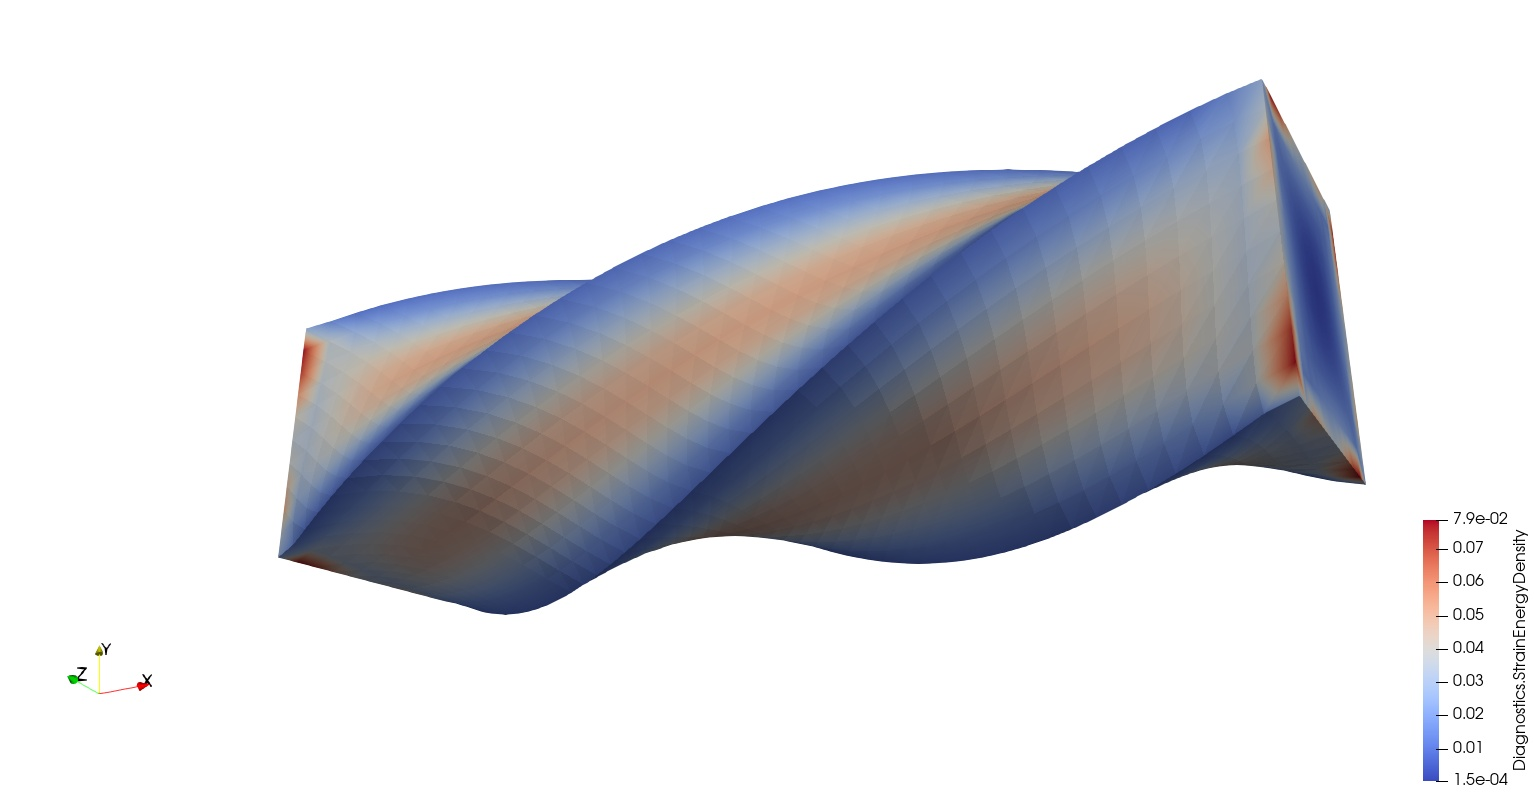
\includegraphics[width=.99\linewidth]{../img/SolidTwistExample}
\caption{Straing Energy Density in Twisted Neo-Hookean Beam}
\label{fig:solidtwist}
\end{figure}

Figure \ref{fig:solidtwist} shows the strain energy density for a beam undergoing a twist with Neo-Hookean hyperelastic modeling at finite strain.
This mini-application can run on host or device processors.
Areas of ongoing research include mixed finite element formulations for the displacement and pressure spaces, efficient load continuation techniques, and preconditioning improvements.
For further information about the libCEED solid mechanics mini-application, see \cite{imece2020} and \cite{mehraban2021simulating}.
